\chapterimage{chapter_head_flauta1.pdf} % Chapter heading image

\chapter{\textcolor{red}{Fundamentos de composição musical}}
Nas seguintes sub seções abordaremos alguns conceitos importantes para iniciar o estudo da dacomposição musical;
porem, não aprofundaremos demasiado em toda a teoria, 
devido a que as explicações mostradas aqui, estão
orientadas para um público interessado na dança, que necesita a principio
ferramentas para entender a musica e melhorar sua percepção musical. 


%%%%%%%%%%%%%%%%%%%%%%%%%%%%%%%%%%%%%%%%%%%%%%%%%%%%%%%%%%%%%%%%%%%%%%%%%%%%%%%%
%%%%%%%%%%%%%%%%%%%%%%%%%%%%%%%%%%%%%%%%%%%%%%%%%%%%%%%%%%%%%%%%%%%%%%%%%%%%%%%%
\section{Articulação}
\label{sub:Articulação}
\index{Música!Articulação}

Nas partituras podemos ver alguns símbolos, 
que o compositor coloca como indicação ao interprete,
para informar como as notas musicais devem ser executadas ou 
articuladas entre sim \cite[pp. 56]{alves2004teoria}.
%%%%%%%%%%%%%%%%%%%%%%%%%%%%%%%%%%%%%%%%%%%%%%%%%%%%%%%%%%%%%%%%%%%%%%%%%%%%%%%%
\subsection{Legato ou ligadura de expressão}
\label{subsec:Legato}
\index{Música!Legato}
O  ``legato'' é um símbolo  que indica uma ligadura de expressão entre as notas,
neste caso a informação que da o compositor é que as
notas devem ser executadas sem interrupções,
criando uma mudança de tons gradual para passar de uma nota musical a outra \cite[pp. 56]{alves2004teoria}.

\begin{example}
A Figura \ref{fig:legato1} mostra um exemplo de uso do legato. 
Alguns instrumentos podem facilmente articular um legato, por exemplo o violino.
\end{example}

\begin{figure}[h!]
\centering
\begin{abc}[name=abc-legato1,width=0.80\linewidth]
X: 1 % start of header
K: C % scale: C major
M: 2/4 %meter - compasso
 (G2 E2 | G1  A1  G1 E1 )|
\end{abc}
\caption{Melodia com notas que devem ser executadas de forma ligada.}
\label{fig:legato1}
\end{figure}

%%%%%%%%%%%%%%%%%%%%%%%%%%%%%%%%%%%%%%%%%%%%%%%%%%%%%%%%%%%%%%%%%%%%%%%%%%%%%%%%
\subsection{Staccato}
\label{subsec:Staccato}
\index{Música!Staccato}

O staccato é um símbolo, desenhado com um ponto (.), 
que indica a diminuição na \hyperref[sec:pos:Duracion]{\textbf{duração}} de uma nota (aproximadamente um 50\%), 
dando nela um efeito de separação ou destaque \cite[pp. 56]{alves2004teoria}.

\begin{example}
A Figura \ref{fig:staccato1a} mostra um exemplo de uso do staccato. 
Na Figura \ref{fig:staccato1b} podemos ver uma escrita equivalente, sem o uso do símbolo de staccato.
\end{example}

\begin{figure}[h!]
\centering
\begin{subfigure}[c]{0.80\textwidth}
\begin{abc}[name=abc-staccato1a]
X: 1 % start of header
K: C % scale: C major
M: 2/4 %meter - compasso
 .G2 .E2 | .G1  .A1  .G1 .E1 | 
\end{abc}
\caption{Notação de notas musicais em staccato.}
\label{fig:staccato1a}
\end{subfigure}
~ %
\begin{subfigure}[c]{1.00\textwidth}
\begin{abc}[name=abc-staccato1b]
X: 1 % start of header
K: C % scale: C major
M: 2/4 %meter - compasso
 G1 z1 E1 z1 | G1/2 z1/2 A1/2 z1/2 G1/2 z1/2 E1/2 z1/2 | 
\end{abc}
\caption{Forma de execução de notas musicais em staccato.}
\label{fig:staccato1b}
\end{subfigure}
\caption{Melodia com notas que devem ser executadas em staccato.}
\label{fig:staccato1}
\end{figure}

\subsubsection{Staccatissimo}

O staccatissimo, staccato seco ou martelado é um símbolo, com uma função similar ao staccato;
porem indica uma diminuição maior na \hyperref[sec:pos:Duracion]{\textbf{duração}} de nota (aproximadamente ao 25\%) \cite[pp. 56]{alves2004teoria}.

\begin{example}
A Figura \ref{fig:staccatissimo1a} mostra um exemplo de uso do staccatissimo. 
Na Figura \ref{fig:staccatissimo1b} podemos ver uma escrita equivalente, sem o uso do símbolo de staccatissimo.
\end{example}

\begin{figure}[h!]
\centering
\begin{subfigure}[c]{0.80\textwidth}
\begin{abc}[name=abc-staccatissimo1a]
X: 1 % start of header
K: C % scale: C major
M: 2/4 %meter - compasso
 !wedge!G2 !wedge!E2 | !wedge!G1  !wedge!A1  !wedge!G1 !wedge!E1 | 
\end{abc}
\caption{Notação de notas musicais em staccatissimo.}
\label{fig:staccatissimo1a}
\end{subfigure}
~ %
\begin{subfigure}[c]{1.00\textwidth}
\begin{abc}[name=abc-staccatissimo1b]
X: 1 % start of header
K: C % scale: C major
M: 2/4 %meter - compasso
 G1/2 z3/2 E1/2 z3/2 | G1/4 z3/4 A1/4 z3/4 G1/4 z3/4 E1/4 z3/4 | 
\end{abc}
\caption{Forma de execução de notas musicais em staccatissimo.}
\label{fig:staccatissimo1b}
\end{subfigure}
\caption{Melodia com notas que devem ser executadas em staccato.}
\label{fig:staccatissimo1}
\end{figure}

%%%%%%%%%%%%%%%%%%%%%%%%%%%%%%%%%%%%%%%%%%%%%%%%%%%%%%%%%%%%%%%%%%%%%%%%%%%%%%%%
\subsection{Tenuto ou sostenuto}
\label{subsec:Tenuto}
\index{Música!Tenuto}

O tenuto é um símbolo, desenhado com uma linha reta (-), 
que indica que deve ser sustentada a 
\hyperref[sec:pos:Duracion]{\textbf{duração}} e a \hyperref[sec:pos:Intensidade]{\textbf{intensidade}} da nota ao máximo \cite[pp. 56]{alves2004teoria}.

\begin{example}
A Figura \ref{fig:tenuto1} mostra um exemplo de uso do tenuto. 
\end{example}


\begin{figure}[h!]
\centering
\begin{abc}[name=abc-tenuto1,width=0.80\linewidth]
X: 1 % start of header
K: C % scale: C major
M: 2/4 %meter - compasso
 !tenuto!G2 !tenuto!E2 | !tenuto!G1  !tenuto!A1  !tenuto!G1 !tenuto!E1 |
\end{abc}
\caption{Melodia com notas que devem ser executadas de forma sustenido.}
\label{fig:tenuto1}
\end{figure}

%%%%%%%%%%%%%%%%%%%%%%%%%%%%%%%%%%%%%%%%%%%%%%%%%%%%%%%%%%%%%%%%%%%%%%%%%%%%%%%%
\subsection{Accénto}
\label{subsec:Accento}
\index{Música!Accénto}

O accénto é um símbolo, desenhado com  (>), 
que indica que a nota deve ser acentuada; 
é dizer, esta deve receber um aumento de \hyperref[sec:pos:Intensidade]{\textbf{intensidade}} \cite[pp. 56]{alves2004teoria}.

\begin{example}
A Figura \ref{fig:accento1} mostra um exemplo de uso do accénto.
Onde os tempos fracos tem um aumento de intensidade provocando \hyperref[sec:contratempo]{\textbf{contratempos}}. 
\end{example}


\begin{figure}[h!]
\centering
\begin{abc}[name=abc-accento1,width=0.80\linewidth]
X: 1 % start of header
K: C % scale: C major
M: 2/4 %meter - compasso
 G2 !>!E2 | G1  !>!A1  !>!G1 !>!E1 |
\end{abc}
\caption{Melodia com notas que devem ser executadas de forma sostenida.}
\label{fig:accento1}
\end{figure}
 
%%%%%%%%%%%%%%%%%%%%%%%%%%%%%%%%%%%%%%%%%%%%%%%%%%%%%%%%%%%%%%%%%%%%%%%%%%%%%%%%
\section{Motivos}
\label{sec:Motivo}
\index{Música!Motivos}
\index{Música!Motif}
\index{Música!Motiv}

Na literatura sobre música podemos achar  termos, motiv (em alemão) ou motif (em inglês),
para designar ao que no português chamaríamos como motivo \cite[pp. 984]{latham2008diccionario}.
Um motivo é uma unidade melódica curta que se repete ao longo de uma composição musical \cite[pp. 545]{apel1969harvard},
esta tem como intenção proporcionar integração, relação, coerência, lógica, 
compreensão e fluidez ao discurso musical \cite[pp. 984]{latham2008diccionario};
sendo estes usados como elementos básicos para a construção
de temas e linhas melódicas \cite[pp. 984]{latham2008diccionario}.

Os motivos são geralmente mais pequenos que um tema ou uma frase,
podendo ter tamanhos tão pequenos quanto só duas notas,
se estas forem o suficientemente representativas \cite[pp. 545]{apel1969harvard}.

%Los *Leitmotiven (motivos principales) de Wagner son el ejemplo más común
%de ideas musicales concisas que además de proporcionar un elemento 
%de estabilidad en la continuidad musical, contribuyen directamente al desarrollo coherente
%de la acción dramática  \cite[pp. 545]{apel1969harvard}.

\begin{example}
Um exemplo muito interessante de uso de motivos pode ser visto na sinfonia n. 5, op. 67, 
de Ludwig van Beethoven.
Na Figura \ref{fig:10Symphony5Op67}, podemos ver os 10 primeiros compassos da sinfonia,
numa versão simplificada que usa só 3 instrumentos, 2 violinos e uma viola.
Nesse fragmento é identificável o motivo nos dois primeiros compassos,
com um conjunto de notas correspondentes a ``sol~sol~sol~mi$\flat$''.
Nos seguintes 3 compassos, o mesmo motivo é usado, 
mas este sofre uma diminuição de 1 tom na altura de todas as notas, 
além de que a última nota musical sofre um amento na sua duração. 
Finalmente nos últimos 5 compassos, cada instrumento por separado sofre uma diferente mutação do motivo;
o violino 1, usa o motivo com um ganho de 8 semitons e um pequeno aumento da ultima nota;
a viola, usa o motivo com um ganho de 13 semitons e um aumento considerável da última nota; e
o violino 2, usa o motivo com um importante aumento na longitude da última nota.
\end{example}


\begin{figure}[!h]
  \centering
    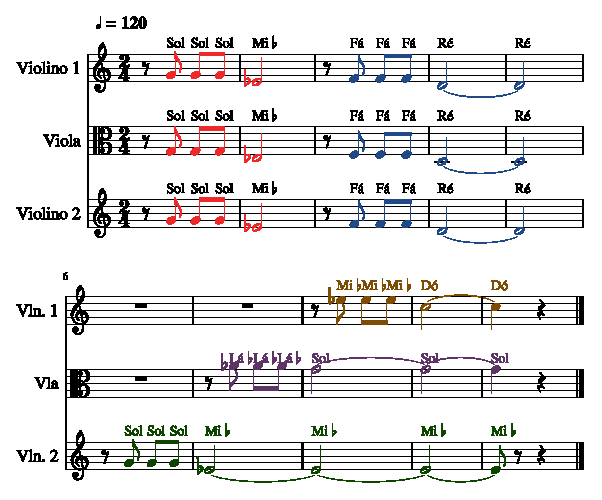
\includegraphics[width=\workboxsize]{chapters/cap-musica-composer/Symphony5Op67-out-1.eps}
\caption{Dez compassos da sinfonia no. 5, op. 67, de Ludwig van Beethoven.}
\label{fig:10Symphony5Op67}
\end{figure}

~


\begin{example}
Na música ``Tico-tico no fubá'' de Zequinha de Abreu, podemos achar exemplos do uso de motivos. 
Na Figura \ref{fig:Tico-tico_no_fuba-1}, temos 5 compassos desta música,
numa versão que usa só 1 instrumentos (um bandolim).
Nesse fragmento é identificável o motivo nos dois primeiros compassos, 
nas 6 primeiras notas musicais, ``mi~ré~mi~fá~mi~lá$\#$''.
imediatamente depois o motivo se repete, porém mudando a ultima nota ate um ``sol$\#$'';
finalmente o motivo volta a parecer, só que além da modificação na altura na ultima nota a um ``ré'',
a duração é encurtada e mais 6 notas musicais são agregadas.
Esta recorrência no uso deste motivo e outros podem ser vistos ao longo de toda a peça musical;
assim, animamo ao leitor a procurar e ouvir a música completa, e tentar identificar o motivo e suas mutações. 
\end{example}

\begin{figure}[!h]
  \centering
    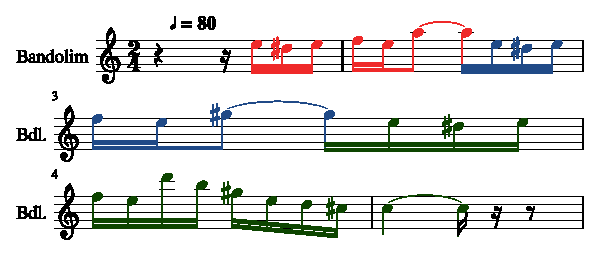
\includegraphics[width=\workboxsize]{chapters/cap-musica-composer/Tico-tico_no_fuba-1.eps}
\caption{Cinco compassos da música ``Tico-tico no fubá'' de Zequinha de Abreu.}
\label{fig:Tico-tico_no_fuba-1}
\end{figure}

~

 
%%%%%%%%%%%%%%%%%%%%%%%%%%%%%%%%%%%%%%%%%%%%%%%%%%%%%%%%%%%%%%%%%%%%%%%%%%%%%%%%
\section{Frase}
\label{sec:Frase}
\index{Música!Frase}
Uma frase é uma unidade musical com sentido e conclusão;
é formada por um grupo de notas que nos dão impressão de que todas pertencem a um mesmo conjunto,
e se caraterizada pela relação entre melodia, ritmo e harmonia,
que termina numa \hyperref[sec:Cadencia]{\textbf{cadência}} \cite[pp. 624]{latham2008diccionario} \cite[pp. 335]{medteoria} \cite[pp. 34]{bennett1993elementos};
é dizer o final da frase pode ser percebido porque a ideia completou o sentido, 
e finaliza num repouso ou uma cadência, além de que a frase seguinte presenta um contraste por estar expressando outra ideia.

\PRLsep{Longitude e usos}

As frases musicais se combinam para formar outras unidades mais longas e completas, 
denominadas \hyperref[sec:Periodo]{\textbf{periodos}} \cite[pp. 624]{latham2008diccionario}.
De forma geral as melodias são construídas usando frases musicais sujeitas a determinadas
regras, de forma similar a como articulamos frases na linguagem falada \cite[pp. 334]{medteoria}.


A longitude de uma frase pode variar, 
porém é comum ver que as frases tem
\begin{itemize}
\item 4 \hyperref[sec:compaso]{\textbf{compassos}} \cite[pp. 624]{latham2008diccionario} \cite[pp. 34]{bennett1993elementos}, 
ou também 
\item 8 compassos  \cite[pp. 335]{medteoria} \cite[pp. 34]{bennett1993elementos};
\end{itemize}
também é comum perceber que as frases que terminam deixando uma sensação de ambiguidade, 
tendem a continuar com outra frase de resposta da mesma longitude \cite[pp. 624]{latham2008diccionario}.


\begin{tcbinformation}
\label{ref:PontoCulminanteSuperior} 
\index{Música!Ponto culminante superior}
\index{Música!PCS}
\index{Música!Clímax}
\textbf{Ponto culminante superior vs. clímax:}
Toda melodia tem uma nota com maior tom (mais aguda), que geralmente está próxima ao final da frase musical;
esta nota é denominada como ponto culminante superior \cite[pp. 336]{medteoria}.
Por outro lado alguns autores fazem uma diferencia entre,
o ponto \textbf{culminante superior} (PCS) e o clímax (Ponto culminante máximo);
onde em cada fragmento da melodia pode ser identificado um PCS,
porém o \textbf{clímax} é a nota mais alta da melodia, como um todo, 
com a característica que a nota é única e está próxima ao final \cite[pp. 12]{melos2012} \cite{HARTMANN2013} \cite[pp. 50]{holland2013music}.
\label{ref:climax}
\end{tcbinformation} 

\PRLsep{Notação}

Na notação musical, 
o compositor pode indicar uma frase, agrupando todas as figuras musicais pertencentes a esta, 
com um símbolo de ligadura escrito acima ou abaixo das notas musicais, 
este simbolo é chamado de ligadura fraseológica \cite[pp. 49]{medteoria} 
\cite[pp. 624]{latham2008diccionario} \cite[pp. 34]{bennett1993elementos}.

A Figura \ref{ritmo:ex2frasesmusicais1} mostra um exemplo de duas frases musicais indicadas pelo uso do simbolo de ligadura.
\begin{figure}[H]
\centering
\begin{abc}[name=abc-ex2frasesmusicais1,options={-O= -c -s 1.5}]
X: 1 % start of header
K: C % scale: C major
M: 4/4 %meter - compasso
V:1 %name="Pauta com clave de fá"   sname="Pauta com clave de fá"
[V:1] (B2 A2 G2 F2| G3 A1 B2 F2) |(C'2 B2 A2 G2| F8)|
\end{abc}
\caption{Duas frases msuicais de 2 compassos cada um.}
\label{ritmo:ex2frasesmusicais1}
\end{figure}

\PRLsep{Estrutura interna}

As frases musicais também podem ser formadas por 2 ou 3 semifrases \cite[pp. 335]{medteoria}.
Com diferencia das frases, que tendem a ser contrastantes; 
as semifrases são identificáveis pois tendem a ser semelhantes entre sim.

\PRLsep{Tipos de frases}

\begin{description}
\item[Frase melódica:]  é uma frase musical formada por um conjunto de tons,
este tipo de frase forma parte de uma linha melódica. 
\item[Frase rítmica:] é uma frase musical formada unicamente por uma distribuição de tempos (ritmo),
este tipo de frase pode ser extraída de um frase melódica, ou servir de base;
também encontraremos frases rítmicas na descrição do ritmo de instrumento de percussão.
\end{description}~

\PRLsep{Frases e texturas musicais}

Na música com \hyperref[subsec:polifonica]{\textbf{textura polifônica}}, 
as frases das diversas linhas melódicas, 
geralmente não finalizam (\hyperref[sec:Cadencia]{\textbf{cadenciam}}) simultaneamente;
por outro lado nas músicas com \hyperref[subsec:homofonica]{\textbf{textura homofônica}},
onde existe uma única linha melódica,
a harmonia de acompanhamento cadência simultaneamente com a melodia \cite{AFraseMelodicaDeterminantes}.

\begin{tcbattention}
Na música contrapontística, é dizer com \hyperref[subsec:polifonica]{\textbf{textura polifônica}}, 
as frases musicais das diferentes vozes se sobrepõem,
com exceção das cadências más importantes onde convergem \cite[pp. 624]{latham2008diccionario}.
\end{tcbattention}

%Na música polifônica há uma distinção maior entre Frase Melódica e Frase estrutural


%%%%%%%%%%%%%%%%%%%%%%%%%%%%%%%%%%%%%%%%%%%%%%%%%%%%%%%%%%%%%%%%%%%%%%%%%%%%%%%%
\subsection{Inicio da frase musical}
\label{subsec:InicioFraseMusical}
O inicio de um ritmo pode ter três formas \cite[pp. 147]{medteoria}:
\begin{itemize}
\item Tético
\item Anacrústico ou protético
\item Acéfalo ou decapitado
\end{itemize}

\subsubsection{Ritmo tético}
\label{subsub:Tetico}
\index{Música!Tético}
É chamado do ritmo tético se este inicia no primeiro tempo do compasso, 
é dizer no tempo forte \cite[pp. 147]{medteoria}.
A Figura \ref{ritmo:iniciotetico1} mostra um exemplo de ritmo tético.
\begin{figure}[H]
\centering
\begin{abc}[name=abc-iniciotetico1]
X: 1 % start of header
K: C % scale: C major
M: 2/4 %meter - compasso
V:1 %name="Pauta com clave de fá"   sname="Pauta com clave de fá"
[V:1] "Compasso 1"G1/2 A B1/2 B1 A1| "Compasso 2"B1 B/2 A/2 G2 |
\end{abc}
\caption{Ritmo tético.}
\label{ritmo:iniciotetico1}
\end{figure}

\subsubsection{Ritmo anacrústico ou protético}
\label{subsub:anacrustica}
\index{Música!Anacrústico}
\index{Música!Protético}
É chamado do ritmo anacrústico ou protético se este inicia antes 
do  tempo forte do compasso \cite[pp. 147-148]{medteoria}.
Na contagem de compassos do ritmo, se diz que este inicia no compasso 1 (primeiro compasso) \cite[pp. 147]{medteoria}.
A Figura \ref{ritmo:anacrustico1} mostra um exemplo de ritmo anacrústico.
\begin{figure}[H]
\centering
\begin{abc}[name=abc-anacrustico1,width=0.8\linewidth]
X: 1 % start of header
K: C % scale: C major
M: 2/4 %meter - compasso
V:1 %name="Pauta com clave de fá"   sname="Pauta com clave de fá"
[V:1]   G1/2 A1/2| "Compasso 1"B1 B/2 A/2 G2 |
\end{abc}
\caption{Ritmo anacrústico.}
\label{ritmo:anacrustico1}
\end{figure}
Não são grafadas as pausas antes da anacruse.
É chamado \textbf{anacruse} às figuras musicais que que estão 
antes do primeiro tempo forte do ritmo, \cite[pp. 148]{medteoria}.
No caso do exemplo da Figura \ref{ritmo:anacrustico1},
a anacruse está formada pelas duas primeiras notas, estas são ``sol~lá''.
Na contagem de compassos do ritmo, se diz que este inicia no compasso 0, 
antes do primeiro compasso \cite[pp. 148]{medteoria}.

Se disse que o ritmo é anacrústico, quando as notas no compasso inicial, 
ocupam menos da metade dele para compassos binários e quaternários,
e menos de dois terços para compassos ternários \cite[pp. 149]{medteoria}.

\subsubsection{Ritmo acéfalo ou decapitado}
\label{subsub:Acefalo}
\index{Música!Acéfalo}
É chamado do ritmo acéfalo ou decapitado quando este inicia numa pausa;
assim, este inicia num tempo fraco \cite[pp. 149]{medteoria}.

Se disse que o ritmo e acéfalo, quando as notas no compasso inicial, 
ocupam mais da metade dele para compassos binários e quaternários,
e mais de dois terços para compassos ternários \cite[pp. 149]{medteoria}.

A Figura \ref{ritmo:acefalo1} mostra um exemplo de ritmo acéfalo.
\begin{figure}[H]
\centering
\begin{abc}[name=abc-acefalo1]
X: 1 % start of header
K: C % scale: C major
M: 2/4 %meter - compasso
V:1 %name="Pauta com clave de fá"   sname="Pauta com clave de fá"
[V:1] "Compasso 1"z F A G1/2 A1/2| "Compasso 2"B1 B/2 A/2 G2 |
\end{abc}
\caption{Ritmo acéfalo.}
\label{ritmo:acefalo1}
\end{figure}

%%%%%%%%%%%%%%%%%%%%%%%%%%%%%%%%%%%%%%%%%%%%%%%%%%%%%%%%%%%%%%%%%%%%%%%%%%%%%%%%
\subsection{Final da frase melódica seguindo o ritmo}
\label{subsec:finaldefrasemus1}
Um ritmo pode ter dois tipos de final, 
masculino e feminino \cite[pp. 150]{medteoria}.

\subsubsection{Frases com final masculino}
\label{subsubsec:finalmasculino}

Se diz que um ritmo tem final masculino, 
quando este termina no tempo forte do compasso \cite[pp. 150]{medteoria}.

A Figura \ref{ritmo:masculino1} mostra um exemplo de frase com final masculino.
\begin{figure}[H]
\centering
\begin{abc}[name=abc-masculino1]
X: 1 % start of header
K: C % scale: C major
M: 2/4 %meter - compasso
V:1 %name="Pauta com clave de fá"   sname="Pauta com clave de fá"
[V:1] z F A G1/2 A1/2| B1 A/2 G1 A1 |F1 z1 z2|
\end{abc}
\caption{Frase com final masculino.}
\label{ritmo:masculino1}
\end{figure}


\subsubsection{Frases com final feminino}
\label{subsubsec:finalfemenino}
Se diz que um ritmo tem final feminino, 
quando este termina em algum tempo fraco do compasso \cite[pp. 150]{medteoria}.

A Figura \ref{ritmo:femenino1} mostra um exemplo de frase com final feminino.
\begin{figure}[H]
\centering
\begin{abc}[name=abc-femenino1]
X: 1 % start of header
K: C % scale: C major
M: 2/4 %meter - compasso
V:1 %name="Pauta com clave de fá"   sname="Pauta com clave de fá"
[V:1] z F A G1/2 A1/2| B1 A/2 G1 A1 |F1 A1 z2|
\end{abc}
\caption{Frase com final femenino.}
\label{ritmo:femenino1}
\end{figure}

%%%%%%%%%%%%%%%%%%%%%%%%%%%%%%%%%%%%%%%%%%%%%%%%%%%%%%%%%%%%%%%%%%%%%%%%%%%%%%%%
\subsection{Final da frase melódica seguindo o acorde de tônica}
\label{subsec:FinalAbertoFechado}
A Tabela \ref{tab:tablefinaltipo} mostra as descrições dos resultados obtidos ao combinar,
o tipo de final rítmico da melodia com o tipo de acorde na cadencia da mesma \cite[pp. 43]{autores2017cuerpo}.

\begin{table}[!h]
  \centering
  \begin{tabular}{|l||p{3cm}|p{2.5cm}|p{3.5cm}|}
  \hline
  ~                      &  \multicolumn{3}{c|}{\textbf{Tipo de acorde na cadência}} \\ \hline
  ~                      & \textbf{Tônica} & \textbf{Outras do acorde de tônica} & \textbf{Fora do acorde de tônica} \\ \hline \hline
  \textbf{F. masculino}  & conclusiva ou afirmativa  & inconclusa & suspensiva ou interrogativa  \\ \cline{1-2}
  \textbf{F. feminino}   & inconclusa                & ~ & ~   \\ \hline
  \end{tabular}  
  \caption{Tipos de final da frase musical seguindo a cadência}
  \label{tab:tablefinaltipo}
\end{table}

\subsubsection{Formula melódica conclusiva ou afirmativa}
É uma formula que dá a sensação de repouso absoluto,
e que tem final masculino  usando a tônica.

\subsubsection{Formula melódica suspensiva ou interrogativa}
É uma formula que dá a sensação de um descanso provisional,
finaliza numa nota que não pertence as notas do ``acorde'' de tônica. 

\subsubsection{Formula melódica inconclusa}
É uma formula que pode finalizar na tônica com final feminino, ou
em outra nota do ``acorde'' de tônica e com final masculino ou feminino.
 
\section{Tema}
\label{sec:tema}
\index{Música!Tema}

O tema ou também denominado sujeito (assunto) ou frase principal,
é o termo que se usa para designar aos passagens melódicos mais importantes de uma obra, 
que conservam um rasgo de continuidade \cite[pp. 411]{stainer2009dictionary} \cite[pp. 1496]{latham2008diccionario}.
Com diferença do termo \hyperref[sec:Motivo]{\textbf{motivo}},
o termo tema é usado para designar a \hyperref[sec:Frase]{\textbf{frases}} completas 
ou \hyperref[sec:Periodo]{\textbf{períodos}} \cite[pp. 1496]{latham2008diccionario},
por outro lado um motivo é muito mais curto e geralmente fragmentário \cite[pp. 545]{apel1969harvard},
para mais detalhes ir a Seção \ref{sec:Motivo}.

O tema é a frase principal de um movimento \cite[pp. 411]{stainer2009dictionary};
porem,  em movimentos em forma de sonata, 
devem existir  dois  temas principais sendo eles os primeiro e o segundo no movimento, e
tem o maior peso estrutural da mesma \cite[pp. 411]{stainer2009dictionary} \cite[pp. 1496]{latham2008diccionario}.

Existem composições politemáticas e monotemáticas;
é dizer com vários temas ou um tema, respectivamente; 
como já vimos, entre os exemplos de composições politemáticas,
temos as sonatas; e como exemplo para composições monotemáticas temos as fugas \cite[pp. 539]{apel1969harvard}.

\begin{example}
Na cultura moderna atual, os temas podem ser mais facilmente reconhecidos  na música cinematográfica.
Por exemplo, para muitos de nós, ficaram marcados os temas dos filmes: ``Superman'', ``Indiana Jones'',
``Star Wars'', ``O grande chefão (The Godfather)'', ``Harry Potter'', etc.
Em algumas ocasiões, os temas podem corresponder aos protagonistas, 
e em outros casos os temas podem fazer referencia a algum elemento na trama.
Porem em todos os casos estão bem gravados na nossa mente, 
de modo que ao escutá-los nos sentimos irreversivelmente obrigados a lembrar seu filme de origem.
\end{example}
 
\section{Período}
\label{sec:Periodo}
\index{Música!Período}



Um período é geralmente formado por duas frases \cite[pp. 350]{duckworth2007creative} \cite[pp. 336]{medteoria};
quando este é o caso 
\begin{itemize}  
\item a primeira é chamada frase antecedente e 
\item a segunda de frase consequente.
\end{itemize}

A frase consequente é uma repetição modificada da frase antecedente 
\cite[pp. 53,55]{schoenberg1990fundamentos} \cite[pp. 25,29]{schoenberg1967fundamentals},
de modo que esta geralmente inicia com o mesmo motivo básico que a frase anterior,
com uma possível leve modificação na melodia
\cite[pp. 51]{schoenberg1990fundamentos} \cite[pp. 25]{schoenberg1967fundamentals};
por outro lado, também é possível que só a estrutura rítmica seja preservada,
e importantes mudanças nas alturas das notas sejam feitas
\cite[pp. 57]{schoenberg1990fundamentos} \cite[pp. 30]{schoenberg1967fundamentals}.


A frase antecedente termina deixando uma sensação de um final aberto, 
que é solucionado pela segunda frase que finaliza com uma cadência conclusiva;
é dizer o período tem duas cadencias uma fraca para a frase antecedente e 
outra forte para a frase consequente 
\cite[pp. 350]{duckworth2007creative} \cite[pp. 336]{medteoria} \cite[pp. 1176]{latham2008diccionario}
\cite[pp. 25,29]{schoenberg1967fundamentals}.

Estas duas frases geram uma analogia literária de pergunta e resposta, respectivamente \cite[pp. 336]{medteoria}.
Comumente, um período é composto por 8 compassos com frases de 4 compassos cada uma \cite[pp. 25]{schoenberg1967fundamentals}.

A Figura \ref{fig:periodostruct} mostra a estrutura de uma período. 
\begin{figure}[!h]
  \centering
    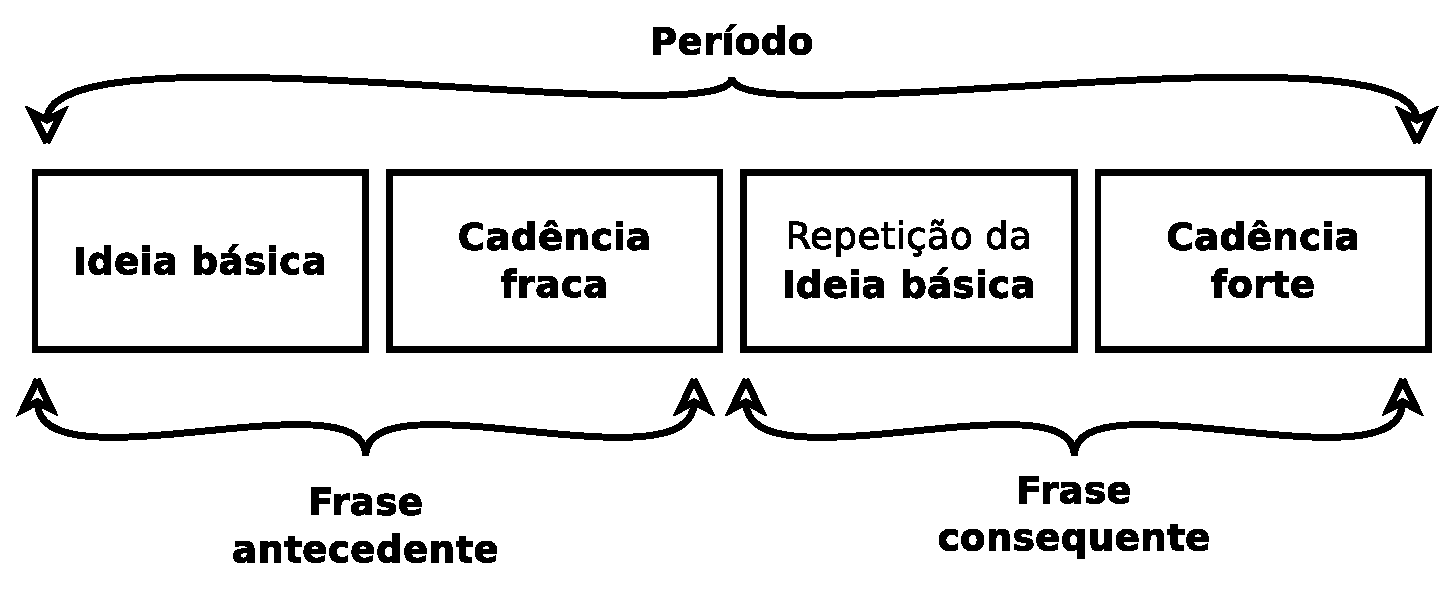
\includegraphics[width=\textwidth]{chapters/cap-musica-composer/periodo.eps}
\caption{Estrutura de uma sentença.}
\label{fig:periodostruct}
\end{figure}

\begin{example}
Na sinfonia no. 9 de Ludwig van Beethoven podemos achar exemplos do uso de períodos. 
Na Figura \ref{fig:periodo-ex1} podemos ver um período formado por 8 compassos desta sinfonia;
os 4 primeiros compassos correspondem à frase antecedente 
e os 4 últimos à frase consequente.
\end{example}

\begin{figure}[!h]
  \centering
    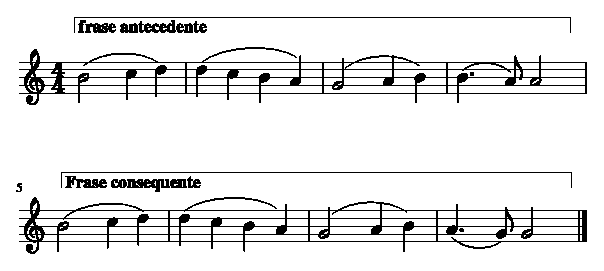
\includegraphics[width=\textwidth]{chapters/cap-musica-composer/periodo-ex1-1.eps}
\caption{Oito compassos da sinfonia no. 9, de Ludwig van Beethoven.}
\label{fig:periodo-ex1}
\end{figure}


 
\section{\textcolor{red}{Sentencia}}\index{Música!Sentencia}
% https://en.wikipedia.org/wiki/Sentence_(music)

\section{\textcolor{red}{Sequencia}}\index{Música!Sequencia}
% https://en.wikipedia.org/wiki/Sequence_(music)

\cite[pp. 763]{apel1969harvard}

\section{\textcolor{red}{Riff}}\index{Música!Riff}
% https://es.wikipedia.org/wiki/Riff
\cite[pp. 1440,1477]{latham2008diccionario}
 
\section{Fraseio}
\label{sec:fraseio}
\index{Música!Fraseio}

O fraseio (frasear) na composição musical, implica  tornar clara e identificável 
o inicio e o final das \hyperref[sec:Frase]{\textbf{frases}} numa peça musical 
mediante o uso adequado de acentuações e cadencias
\cite[pp. 336]{medteoria} \cite[pp. 19]{holst1998abc}.
Anteriormente, 
o fraseio na música era deixado para ser escolhido livremente pelo sentido de bom senso e gosto de cada intérprete;
porém, atualmente é comum que os compositores modernos usem vários simbolos para indicar o fraseio \cite[pp. 348]{stainer2009dictionary}.
Assim, as frases são separadas na pauta usando signos como a \hyperref[fig:Cesura]{\textbf{cesura}}\footnote{Para
 mais detalhes ir a Pagina \pageref{fig:Cesura}.}  \cite[pp. 668]{apel1969harvard},
que serve para que o interprete recupere o folego 
antes da seguinte frase musical \cite[pp. 18]{holst1998abc} \cite[pp. 48]{howard1991aprendendo},
da mesma forma que acontece com o signos de pontuação na leitura de um discurso.




\begin{figure}[!h]
\begin{elaboracion}{Cesura}
\index{Música!Cesura}
A cesura é um simbolo que indica uma pequena pausa entre duas frases,
é equivalente a dizer que a ultima nota da primeira frase terá uma diminuição pequena, só para pegar folego;
entre os símbolos usados para a cesura temos a virgula ``\textbf{,}'' 
ou também uma ``\textbf{v}'', ou ``\textbf{//}'', ou ``\textbf{/}'' 
\cite[pp. 252]{medteoria} \cite[pp. 18]{holst1998abc}.
A seguinte figura mostra o uso da cesura, na qual é indicado que o interprete deverá 
dar uma pausa na última nota da primeira frase, neste caso diminuindo a duração da nota sol.\\
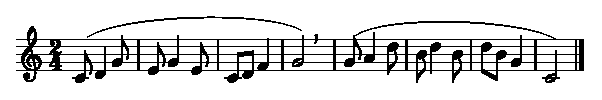
\includegraphics[width=\textwidth]{chapters/cap-musica-topicos/cesura1-1.eps}
\end{elaboracion}
\label{fig:Cesura}
\end{figure}
 
Por outra lado, para os executantes da música, 
o fraseamento é a arte de interpretar as frases individuais ou elas em conjunto numa composição musical;
sendo este ponto 
uma caraterística importante da estética particular que dá cada interprete à música 
\cite[pp. 257]{medteoria} \cite[pp. 624]{latham2008diccionario}.
Falando em termos mais rigorosos, 
o fraseado na interpretação refere-se à separação de uma melodia na suas frases constituintes 
\cite[pp. 668]{apel1969harvard}.

Uma caraterística interessante da música, 
é que o comprimento das frases é influenciado diretamente pela capacidade respiratória do ser humano,
mesmo em instrumentos que não são de sopro como o piano \cite[pp. 48]{howard1991aprendendo},
isto poderia dever-se a que nos sentimos mais confortáveis de escutar composições musicais,
que relacionamos facilmente com um discurso falado.

\begin{example}
Leia  o seguinte texto respeitando acentos, descansos e signos de admiração e interrogação:
\begin{citando}%%
Boa tarde amigo!\\
Como você está?\\
Bem, muito obrigado.
\end{citando}%%

Agora, com a ajuda de um piano, execute a melodia mostrada na Figura \ref{fig:conversa1},
e tente respeitar o mesmo fraseio que no texto, se ajude usando as ligaduras de expressão e a cesura.
\end{example}

\begin{figure}[!h]
\centering
\href{https://drive.google.com/file/d/1rOD08xWn0m5R2KPRa2gf3ycU0nF7sOgV/view?usp=sharing}{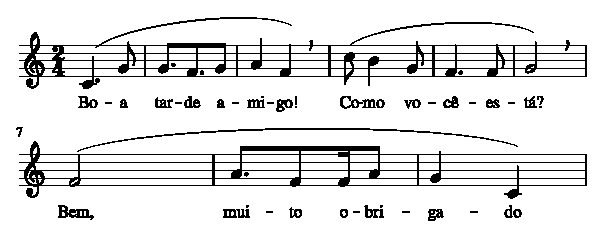
\includegraphics[width=\textwidth]{chapters/cap-musica-topicos/conversa-1.eps}}
\caption{Frases musicais.}
\label{fig:conversa1}
\end{figure}

% https://es.wikipedia.org/wiki/Fraseo
% https://en.wikipedia.org/wiki/Musical_phrasing


 
%%%%%%%%%%%%%%%%%%%%%%%%%%%%%%%%%%%%%%%%%%%%%%%%%%%%%%%%%%%%%%%%%%%%%%%%%%%%%%%%
\section{Cadência}
\label{sec:Cadencia}
\index{Música!Cadência}

\begin{tcbinformation}{Música cadenciosa}
\index{Música!Música cadenciosa}
\label{ref:musicacadenciosa}
É aquela que tem um ritmo facilmente apreciável, na qual as terminações, ou seja cadências,
são fáceis de perceber \cite[pp. 60]{pedrell2009diccionario}.
Para que uma música seja cadenciada é preciso que ritmo e harmonia se combinem  
para dar uma sensação de exatidão \cite[pp. 68]{melcior1859diccionario}.
\end{tcbinformation} 


O final da frase musical está marcado pela cadência, 
este nome vem da palavra ``cadenza''  em italiano que significa caindo ou cessando \cite[pp. 34]{bennett1993elementos} \cite[pp. 68]{melcior1859diccionario}. 
As cadências existem nas frases melódicas ou harmônicas, 
e são identificáveis como os períodos de repouso entre as frases musicais;
estas cumprem o mesmo papel que os signos de pontuação na gramática, 
já seja como virgulas, pontos e virgulas, pontos, signos de interrogação
\cite[pp. 66,67]{melcior1859diccionario} \cite[pp. 34]{bennett1993elementos}, 
etc.


%%%%%%%%%%%%%%%%%%%%%%%%%%%%%%%%%%%%%%%%%%%%%%%%%%%%%%%%%%%%%%%%%%%%%%%%%%%%%%%%
\subsection{Cadência harmônica}
\label{sec:CadenciaHarmonica}
\index{Música!Cadência harmônica}

As cadencias harmônicas estão representadas por um par de ``acordes''
que são usados para finalizar uma frase musical, estas tem um sentido de mensagem. 

Entre os tipos de cadencias harmônicas, 
temos as que nos dão a liberdade expressar uma pausa momentânea, suspenso ou o final de uma ideia.

A Tabela \ref{tab:tiposdecadencia} mostra algumas desta opções, 
na primeira coluna temos os nomes dos tipos de cadencias,
na segunda coluna temos a ordem e os graus dos acordes que são usados para gerar essa cadência 
e na terceira coluna está a descrição de cada um dos tipos de cadência.

\begin{table}[h]
  \centering
  \begin{tabular}{|p{4cm}|l|p{8cm}|}
  \hline
  Nome & Acordes   & Analogia \\ \hline
  \hline
  Cadência perfeita & V-I       & Dá sentido de algo perfeitamente acabado, 
  equivalente a um ponto final na gramática \cite[pp. 34]{bennett1993elementos}. \\ \hline
  
  Cadência plagal   & IV-I      & Dá um sentido equivalente a um ponto final na gramática, 
  também é chamado de cadência do ``Amém'' 
  por seu uso em hinos religiosos \cite[pp. 34]{bennett1993elementos} \\ \hline

  Cadência imperfeita ou semicadência \cite[pp. 103]{grabner2001teoria} & ?-V    & Acontece quando se vá de um grau qualquer para finalizar na dominante (V), 
  porém é comum ver que se usam:
  I-V,II-V e IV-V. Esta cadência dá à música a sensação de um final incompleto, 
  seu efeito é similar ao de uma virgula na gramática,
  \cite[pp. 34]{bennett1993elementos}. \\ \hline

  Cadência interrompida & V-($\neq$I) & Acontece quando se sugere que acontecerá uma cadencia V-I (dominante-tônica),
  porém apos V se finaliza em qualquer grau 
  diferente da \hyperref[sec:Tonica]{\textbf{tônica}}, geralmente VI,
  e dá uma sensação de surpresa e de interrupção à música; ou seja uma frase incompleta.
  \cite[pp. 35]{bennett1993elementos}. \\ \hline  
\end{tabular}
  \caption{Tipos de cadência harmônica.}
  \label{tab:tiposdecadencia}
\end{table}

\begin{example}
A Figura \ref{fig:abc-perfeita1} mostra uma cadência perfeita para uma tônica em acorde de dó.
A cadência dá a sensação de uma frase com ponto final.
\end{example}

\begin{figure}[H]
\centering
\begin{abc}[name=abc-perfeita1,width=1.0\linewidth]
X: 1 % start of header
K: C % scale: C major
M: 2/4 %meter - compasso
V:1 %name="Pauta com clave de fá"   sname="Pauta com clave de fá"
[V:1] | [C2 E2 G2] [F2 A2 C'2]| [E2 G2 B2] [G2 B2 D'2]| [F2 A2 C'2] [G2 B2 D'2]| [C2 E2 G2] z2|
w: ~ ~ ~ ~ ~ V I
\end{abc}
\caption{Cadência perfeita.}
\label{fig:abc-perfeita1}
\end{figure}

\begin{example}
A Figura \ref{fig:abc-plagal1} mostra uma cadência plagal para uma tônica em acorde de dó.
A cadência dá a sensação de uma frase com ponto ao  final.
\end{example}

\begin{figure}[H]
\centering
\begin{abc}[name=abc-plagal1,width=1.0\linewidth]
X: 1 % start of header
K: C % scale: C major
M: 2/4 %meter - compasso
V:1 %name="Pauta com clave de fá"   sname="Pauta com clave de fá"
%[V:1] | [E2 G2 B2] [F2 A2 C'2]| [E2 G2 B2] [G2 B2 D'2]| [C2 E2 G2] z2|
[V:1] | [C2 E2 G2] [F2 A2 C'2]| [E2 G2 B2] [G2 B2 D'2]| [E2 G2 B2] [F2 A2 C'2]| [C2 E2 G2] z2|
w: ~ ~ ~ ~ ~ IV I
\end{abc}
\caption{Cadência plagal.}
\label{fig:abc-plagal1}
\end{figure}

\begin{example}
A Figura \ref{fig:abc-imperfeita1} mostra uma cadência imperfeita para uma tônica em acorde de dó.
A cadência dá a sensação de uma frase com um final débil, como de uma mistura de signo de admiração e interrogação.
\end{example}

\begin{figure}[H]
\centering
\begin{abc}[name=abc-imperfeita1,width=1.0\linewidth]
X: 1 % start of header
K: C % scale: C major
M: 2/4 %meter - compasso
V:1 %name="Pauta com clave de fá"   sname="Pauta com clave de fá"
[V:1] | [C2 E2 G2] [F2 A2 C'2]| [E2 G2 B2] [G2 B2 D'2]| [E2 G2 B2] [F2 A2 C'2]| [G2 B2 D'2] z2|
w: ~ ~ ~ ~ ~ IV V
\end{abc}
\caption{Cadência imperfeita.}
\label{fig:abc-imperfeita1}
\end{figure}


\begin{example}
A Figura \ref{fig:abc-interrompida1} mostra uma cadência interrompida para uma tônica em acorde de dó.
A cadência dá a sensação de uma frase incompleta.
\end{example}

\begin{figure}[H]
\centering
\begin{abc}[name=abc-interrompida1,width=1.0\linewidth]
X: 1 % start of header
K: C % scale: C major
M: 2/4 %meter - compasso
V:1 %name="Pauta com clave de fá"   sname="Pauta com clave de fá"
[V:1] | [C2 E2 G2] [F2 A2 C'2]| [E2 G2 B2] [G2 B2 D'2]| [E2 G2 B2] [G2 B2 D'2]| [A2 C'2 E'2] z2|
w: ~ ~ ~ ~ ~ V VI
\end{abc}
\caption{Cadência interrompida.}
\label{fig:abc-interrompida1}
\end{figure}

%%%%%%%%%%%%%%%%%%%%%%%%%%%%%%%%%%%%%%%%%%%%%%%%%%%%%%%%%%%%%%%%%%%%%%%%%%%%%%%%
\subsection{Cadência melódica} 
\label{subsec:cadenciamelodica}
Quando nos referimos à forma em que uma melodia é finalizada,
estamos falando da cadencia melódica; esta pode ser categorizada em: 
\begin{itemize}
\item \textbf{Cadências}, se o repouso é equivalente a um ponto na gramática \cite[pp. 66,67]{melcior1859diccionario},
como o produzido por uma dominante (V) seguida de um tônica (I).
\item \textbf{Semicadências}, se repouso é equivalente a um ponto e virgula na gramática \cite[pp. 66,67]{melcior1859diccionario};
esta também é chamada de cadencia imperfeita e se carateriza por terminar numa dominante (V) 
que geralmente vem precedida por  I, II ou IV \cite[pp. 103]{grabner2001teoria}; 
é possível ver este tipo de cadencia no final da frase antecedente de um 
\hyperref[sec:Periodo]{\textbf{período}} \cite[pp. 21]{latham2008diccionario}.
\item \textbf{Quartos de cadência}, se o repouso é igual a uma virgula \cite[pp. 66,67]{melcior1859diccionario}.
\end{itemize}~

Todas estas cadencias dão à melodia uma sensação da conclusão de uma ideia; 
porém, cada uma destas nos deixa uma perspetiva diferente sobre o que vem depois e quando.

Além dos tipos de cadencias melódicas anteriormente mencionadas, podemos achar também a:
\begin{itemize}
\item \textbf{Cadência interrompida}, este tipo de cadencia se verifica 
quando ao final de um período sugerimos que iremos de 
\hyperref[sec:dominante]{\textbf{dominante}} a \hyperref[sec:Tonica]{\textbf{tônica}},
porém terminamos em qualquer outro grau; ou seja pulamos da dominante a um grau diferente da tônica 
\cite[pp. 67]{melcior1859diccionario} \cite[pp. 60]{pedrell2009diccionario}. 
\end{itemize}~

Em geral veremos um uso aprimorado das cadências, na frase consequente de um \hyperref[sec:Periodo]{\textbf{período}},
onde o tipo do cadência ajudará a expressar o uso que esta terá na peça musical  \cite[pp. 66,67]{melcior1859diccionario}.

\begin{example}
A Figura \ref{fig:abc-frasemelodica1} mostra duas frases com tônica em dó, 
a primeira frase com uma semicadencia (VI-V) e a segunda frase com uma cadência (V-I).
\end{example}

\begin{figure}[H]
\centering
    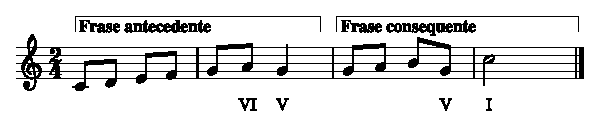
\includegraphics[width=\textwidth]{chapters/cap-musica-composer/frasemelodica1-1.eps}
\caption{Duas frases melódicas com tônica em dó.}
\label{fig:abc-frasemelodica1}
\end{figure}

\begin{example}
A Figura \ref{fig:abc-frasemelodica2} mostra duas frases  com tônica em sol, 
a primeira frase com uma cadência interrompida (V-III) e a segunda frase com uma cadência (V-I).
\end{example}

\begin{figure}[H]
\centering
    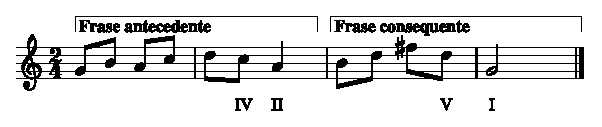
\includegraphics[width=\textwidth]{chapters/cap-musica-composer/frasemelodica2-1.eps}
\caption{Duas frases melódicas com tônica em sol.}
\label{fig:abc-frasemelodica2}
\end{figure}
% https://es.wikipedia.org/wiki/Cadencia_(música)

% https://en.wikipedia.org/wiki/Cadence

 
\section{Tensão e liberação }
\index{Música!Tensão}

\subsection{O que é tensão}
Ao escutar uma porção de uma peça musical, percebemos que esta provoca na nossa mente
um sentido de antecipação.
Esta percepção nos conduz, internamente, 
a ter um estado variável entre a tensão (expetativa ou ``tension'' em inglês)
ou um sentido de liberação (resolução, descanso, ou ``release'' em inglês).
Assim podemos descrever à tensão como o 
estado onde sentimos a necessidade de obter uma resolução; e dizer, passar a um estado de liberação.
Em muitas ocasiões o compositor usa este recurso para chamar nossa atenção,
deixando-nos impacientes para obter uma resposta. 
Quanto tempo o compositor vai nos torturar esperando a resposta, 
é uma liberdade criativa de cada artista.

\begin{example}
Um exemplo onde é muito fácil perceber o uso da tensão na música, 
para comunicar estados de animo no espectador, 
pode ser escutado no tema principal da banda sonora do filme ``Jaws'' (Tubarão) 1975,
escrita por John Williams\footnote{Este tema é fácil de achar usando as palavras chave:``Jaws main theme soundtrack''.}.

Ao escutar a peça musical automaticamente entraremos num percorrido que nos leva lentamente,
porem sem pausa, a um estado de tensão e suspense, seguido de um pequeno momento de calma,
que cumpre a função de dar-nos uma falsa sensação de paz,
 para logo nos surpreender com um estado de tensão ainda maior;
finalizando o tema num estado de liberação (calma).
\end{example}

\subsection{Como se modifica a tensão?}

Alguns compositores e artistas dividem a obtenção da tensão, em dois grandes grupos \cite{edmtensionrelease1}:
\begin{itemize}
\item \textbf{Macro-tensão:}
é uma tensão que se trabalha durante um período de tempo longo. 
Onde a tensão vai se acumulando para servir de transição entre uma parte do arranjo para outra;
ou também a tensão pode diminuir ao longo do tempo ate chegar a um ponto de baixa energia.
Normalmente, uma macro-tensão é usada para fazer a transição a uma queda, coro, ponte \cite{edmtensionrelease1}, etc.
\item \textbf{Micro-tensão:}
são  quebras isoladas do padrão, que acontecem de forma pontual ao longo da peça musical, 
como alterações na melodia, breques, acordes não resolvidos, etc. 
Em geral pode se referir a qualquer coisa que altere pontualmente a monotonia da peça musical \cite{edmtensionrelease1}.
\end{itemize}~

O aumento ou a diminuição da tensão na música pode ser promovido por vários fatores; 
sendo que este efeito pode ser pontual ou trabalhado ao longo de uma seção.
para compreender melhor como este aspecto da música  é controlado,
 a continuação são listados alguns dos fatores que contribuem à modificação da tenção:
\begin{itemize}
\item o tom \cite[pp. 3]{wright2012essential},
\item a intensidade (volume) \cite[pp. 3]{wright2012essential},
\item a dissonância \cite[pp. 28-29]{kerman2015listen} \cite[pp. 26]{wright2012essential},
\item o ritmo, 
\item as cadencias nas frases musicais,
\item etc.
\end{itemize}~

Para ter uma ideia mais clara de como estes elementos provocam tensão podemos usar a Tabela  \ref{tab:tensionrelease1}.  
\begin{table}[h]
  \centering
  \begin{tabular}{| p{3cm} || p{3.0cm} | p{3.0cm} |}
   \hline 
   Tipo & Tensão     & Relaxação \\ \hline 
   \hline 
   Tom          & Incremento & Diminuição  \\ \hline
   Intensidade  & Incremento & Diminuição  \\ \hline
   Dissonância  & Incremento & Diminuição  \\ \hline
   Ritmo        & Incremento da velocidade & Diminuição da velocidade \\ \hline
   Cadência     & Final aberto & Final fechado \\ \hline
  \end{tabular}
  \caption{Tensão e relaxação na música.}
  \label{tab:tensionrelease1}
\end{table}
Onde na primeira coluna  vemos a caraterística em estudo,
a segunda coluna nos indica que debemos fazer com essa caraterística para aumentar a tensão,
e a terceira coluna nos indica que devemos fazer com a caraterística para diminuir a tensão;
é dizer aumentar a relaxação.

%%%%%%%%%%%%%%%%%%%%%%%%%%%%%%%%%%%%%%%%%%%%%%%%%%%%%%%%%%%%%%%%%%%%%%%%%%%%%%%%
\begin{example}[Tensão pela mudança do tom:]
A Figura \ref{fig:tension-release-tom-1} mostra como podemos incrementar e diminuir a tensão,
pelo aumento e a diminuição do tom. 
Nos 4 primeiros compassos a tensão cresce com o aumento do tom,
e nos 4 últimos compassos a tensão diminui com a diminuição do tom.
\end{example}
\begin{figure}[!h]
     \centering
     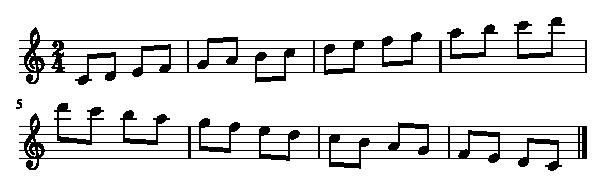
\includegraphics[width=1.0\textwidth]{chapters/cap-musica-topicos/tension-release-tom-1.eps}
     \caption{Incremento e diminuição por mudança do tom.}
     \label{fig:tension-release-tom-1}
\end{figure}


%%%%%%%%%%%%%%%%%%%%%%%%%%%%%%%%%%%%%%%%%%%%%%%%%%%%%%%%%%%%%%%%%%%%%%%%%%%%%%%%
\begin{example}[Tensão pela mudança de intensidade:]
A Figura \ref{fig:tension-release-intensidade-1} mostra como podemos incrementar e diminuir a tenção,
pelo aumento e a diminuição da intensidade. 
Nos 4 primeiros compassos a tensão cresce com o aumento da intensidade,
e nos 4 últimos compassos a tensão diminui com a diminuição da intensidade.
\end{example}
\begin{figure}[!h]
     \centering
     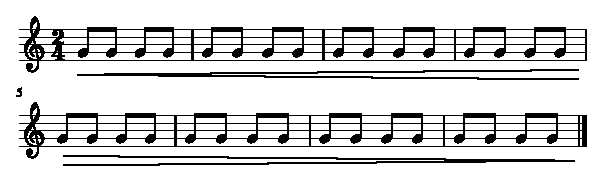
\includegraphics[width=1.0\textwidth]{chapters/cap-musica-topicos/tension-release-intensidade-1.eps}
     \caption{Incremento e diminuição por mudança na intensidade.}
     \label{fig:tension-release-intensidade-1}
\end{figure}


%%%%%%%%%%%%%%%%%%%%%%%%%%%%%%%%%%%%%%%%%%%%%%%%%%%%%%%%%%%%%%%%%%%%%%%%%%%%%%%%
\begin{example}[Tensão pelo uso de dissonâncias:]
A Figura \ref{fig:tension-release-dissonancia-1} mostra como podemos incrementar e diminuir a tenção,
pelo aumento e a diminuição da dissonância. 
Nos 4 primeiros compassos a tensão cresce com o aumento da dissonância,
e nos 4 últimos compassos a tensão diminui com a diminuição da dissonância.
\end{example}
\begin{figure}[!h]
     \centering
     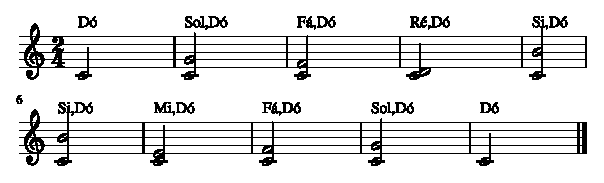
\includegraphics[width=1.0\textwidth]{chapters/cap-musica-topicos/tension-release-dissonancia-1.eps}
     \caption{Incremento e diminuição por mudança na dissonância.}
     \label{fig:tension-release-dissonancia-1}
\end{figure}


%%%%%%%%%%%%%%%%%%%%%%%%%%%%%%%%%%%%%%%%%%%%%%%%%%%%%%%%%%%%%%%%%%%%%%%%%%%%%%%%
\begin{example}[Tensão pela mudança de ritmo:]
A Figura \ref{fig:tension-release-ritmo-1} mostra como podemos incrementar e diminuir a tenção,
pelo aumento e a diminuição da velocidade no ritmo. 
Nos 4 primeiros compassos a tensão cresce com o aumento da velocidade do ritmo,
e nos 4 últimos compassos a tensão diminui com a diminuição da velocidade do ritmo.
\end{example}
\begin{figure}[!h]
     \centering
     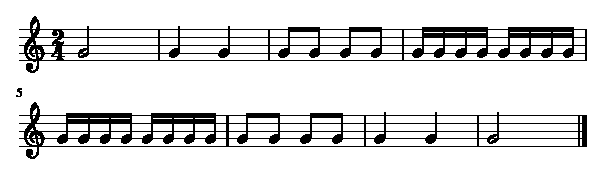
\includegraphics[width=1.0\textwidth]{chapters/cap-musica-topicos/tension-release-ritmo-1.eps}
     \caption{Incremento e diminuição por mudança na intensidade.}
     \label{fig:tension-release-ritmo-1}
\end{figure}

\begin{example}[Tensão pela uso de cadências:]
Para incrementar e diminuir a tenção numa peça musical pelo uso de cadências nas frases musicais,
devemos seguir os tipos de finalizações explicados na Seção \ref{sec:Cadencia}.
Por exemplo, fazendo um paralelo com as frases (gramaticais),
teremos uma expetativa diferente numa frase finalizada de forma enunciativa (``faz frio'') 
que uma frase interrogativa (``Faz frio?''), 
onde a primeira frase nos deixa num estado de relaxação (liberação),
enquanto que a segunda nos deixa uma expetativa (tensão) 
que procura ou espera obter depois uma resposta (resolução).  
\end{example}

% 
% https://www.schoolofcomposition.com/what-is-tension-and-release-in-music/
% https://www.youtube.com/watch?v=613v8nbsWFY
% https://www.youtube.com/watch?v=5kYZmQzMxD0


